\section{Durchführung}
\label{sec:Durchführung}
\subsection{Aufbau der Apparatur}
Gemessen wird mit einer Ultraschallsonde mit einer Frequenz von $2\si{\mega\hertz}$, ein
Rechner mit dem Programm FlowView dient der Datenanalyse. Gemessen wird an einem System aus Ströhmungsröhren mit unterschiedlichem
Durchmesser, durch diese wird mittels regelbarer Zentrifugalpumpe eine Flüßigkeit geleitet. Zur Kopplung der Sonde an eine der Röhren dient ein Doppler-Prisma,
dieses besitz drei Flächen, die einen Prismenwinkel von $15^°$, $30^°$ und $60^°$ zwischen Sonde und strömenden Flüssigkeit einstellen.

\subsection{Durchführung}
\label{sec:durch}
Bei der ersten Messung werden die Strömungsgeschwindigkeiten in Abhängigkeit zum Dopplerwinkel gemessen. Dazu wird die Sonde auf eine der Prismenflächen gelegt und am Computer die Werte Speed und
f-mean (siehe Abbildung \ref{fig:bsp} abgelesen. F-mean bedeutet $\Delta\nu$ und Speed die Geschwindigkeit $v$.
Dieser Vorgang wird für fünf verschiedene Flüßigkeiten und alle drei Prismenwinkel wiederholt. Das Sample Volume wird beim Generator auf Large gestellt.
\begin{figure}
  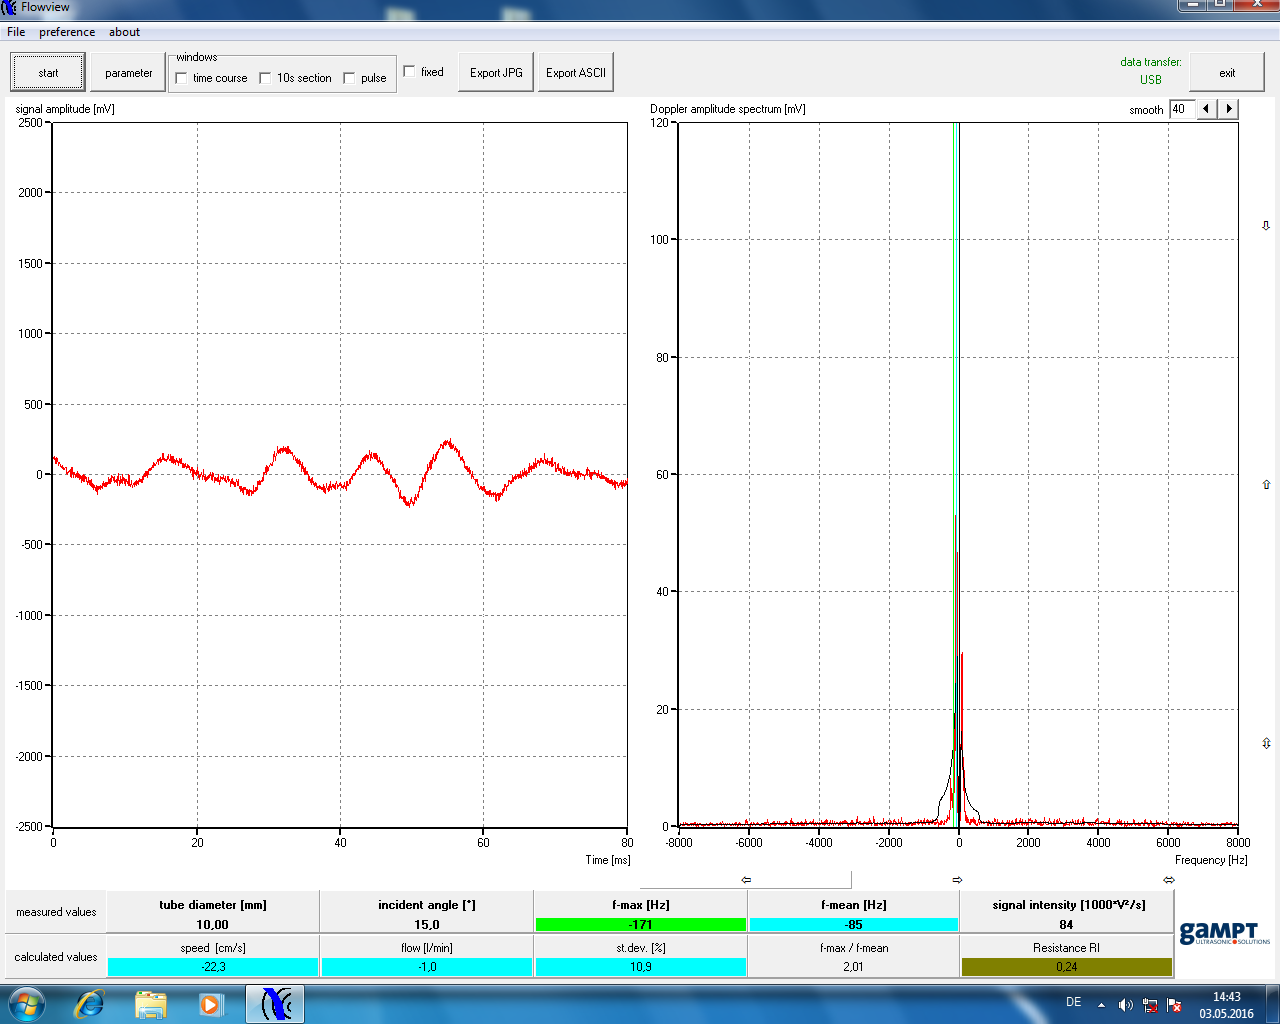
\includegraphics[width=0.7\textwidth]{Unbenannt.png}
  \centering
   \caption{Bild des Programm-Layouts }
  \label{fig:bsp}
\end{figure}

Die zweite Messung dient zur Profilanalyse der Strömung,
gemessen wird an einer der Röhren mit einem Prismenwinkel von $15^°$ und einer
Fließgeschwindigkeit von ca.$60\%$ und ca.$40\%$.
Das Sample Volume wird auf Small gestellt und mit dem Depth-Regler wird die Tiefe variiert.
Aufgenommen wurden die Werte Speed und Signal Intensity (siehe Abbildung \ref{fig:bsp}), was dem Streuintensitätswert entspricht.
